\subsection{Formulating a Neural Network model for Continuous-Time Processes}

In the following discussion, we only worry about time-independent (sometimes also refered to as autonomous) systems, as those are more relevant for control, but most of those approaches generalize well to time-dependent systems as well. Time-Continuous Neural Networks model dynamical systems model the evolution of the hidden states (which we denote as $\bm{x}_t$ at a given time $t$) of a neural network by equations of the form: 

\begin{align}
    \frac{\partial \bm{x}_t}{\partial t} = D(\bm{x}_t, \bm{I}_t, \theta, A).
\end{align}
 
 Where $D$ denotes some kind of model function that estimates the time-derivative of $\bm{x}_t$. $D$ is a function of $\bm{x}_t$, which denotes the hidden state of the neuron, $\bm{I}_t$ which denotes the inputs of the neuron, a fixed parameter vector $A$ and a learnable parameter vector $\theta$. Updates of the (hidden) state $\bm{x}_t$ are the computed using some ODE solver which integrates $\frac{\partial \bm{x}_t}{\partial t}$ over some time-step $\Delta t$ to compute $\bm{x}_{t+\Delta t} = \int_t^{t+\Delta t} \frac{\partial \bm{x}_t}{\partial t} + \bm{x}_t$.
 
 
 \begin{align}
    D(\bm{x}_t, \bm{I}_t, \theta, A) =  f(\bm{I}_t, \theta, A).
\end{align}
 
 It is worth noting that in a supervised learning context, this formulation has the advantage of being able to represent irregularly sampled time-sequences. For the control applications we consider here, the sample-rate is imposed by the hardware of our robot and is likely regular. In the original formulation of Chen et al, neural ODEs are not recurrent but a natural extension to recurrent neural networks can be formulated as: \\

 \begin{align}
    D(\bm{x}_t, \bm{I}_t, \theta, A) =  f(\bm{x}_t, \bm{I}_t, \theta, A).
\end{align}
 
Where the flow $D$ is not only a function of the input $\bm{I}_t$ but also of the inner-state $\bm{x}_t$. Such a model can be though of as a recurrent neural network where the recurrent connection are implemented by an integrator.

\begin{figure}[h!]
    \centering
    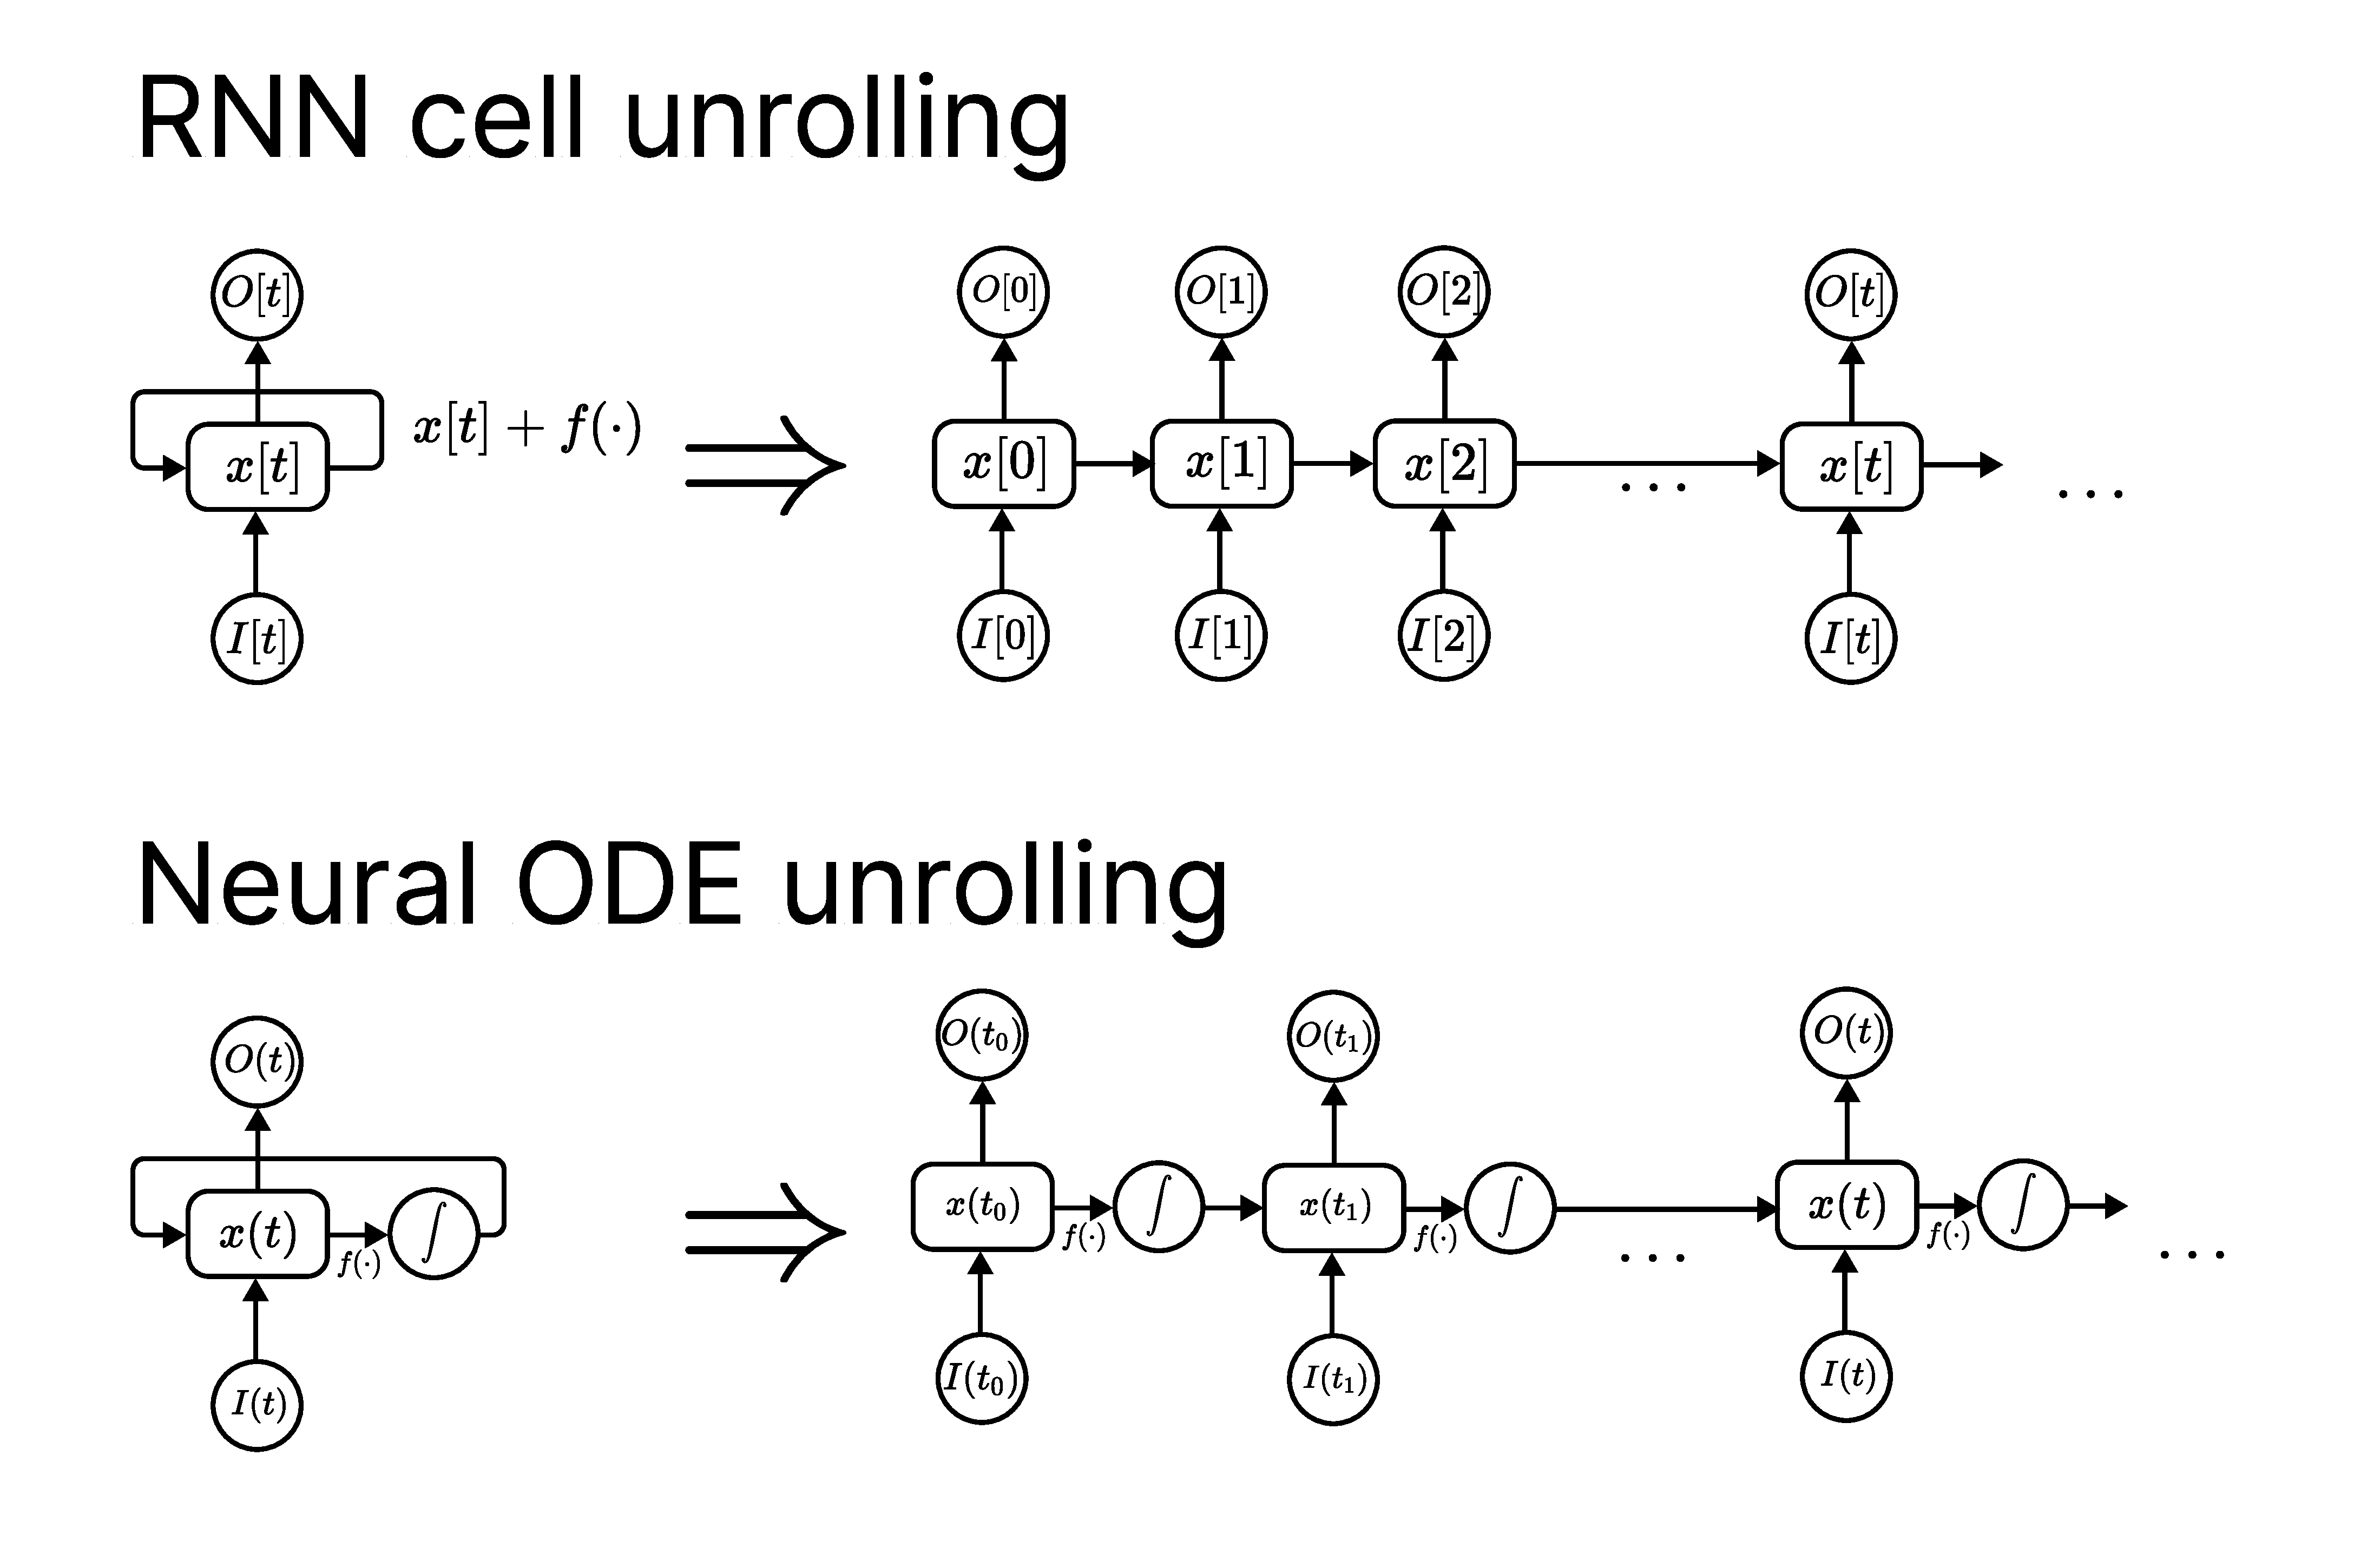
\includegraphics[width=0.45\textwidth]{figures/unroll.pdf}
    \caption{An illustration of the difference between Neural ODE unrolling v.s. RNN unrolling.}
\end{figure}

 The most straight forward approach to that problem is directly using a neural network to model the flow $D$, this is the approach chosen by \cite{Chen2018NeuralOD} (which is often referred to as "Neural-ODEs"). An alternative provided by an earlier contribution is the so called "Continuous-Time Recurrent Neural Network" model (CT-RNNs) first proposed by Funahashi and Nakamura in \cite{Funahashi1993ApproximationOD}, which pick $D$ as: 
 
\begin{align}
    D(\bm{x}_t, \bm{I}_t, \theta, A) = -\frac{\bm{x}_t}{\tau} + f(\bm{x}_t, \bm{I}_t, \theta, A).
\end{align}

where $\tau$ is a fixed time constant (according to our formalism it is an element of the vector $A$) and $f$ a non-linear activation function. The fixed time-constant is is introduced to induce a decay in the behavior of the neurons which is meant to enable recurrent connections which avoiding unstable neuron dynamics. In their original paper, Funahashi and Nakamura propose to use $f = \sum_{j=1}^m w_{i,j} \cdot \sigma\left( x_{i,t} \right) + I_i (t)$, where the weights $w{i,j}$ are elements of the vector $\theta$. \\

More recently, one suggested implementation that seems to give better performance is proposed by Hasani and Lechner though so-called "Liquid Time-Constant networks (LTCs)" \cite{Hasani2021LiquidTN}. In that case the activation $f$ affects both the time-constant and the non-linearity (hence make the time-constant "liquid"), this approach corresponds to the following time-derivative model:

\begin{align}
    D(\bm{x}_t, \bm{I}_t, \theta, A) = - \left[ \frac{1}{\tau} + f(\bm{x}_t, \bm{I}_t, \theta, A) \right] \bm{x}_t \nonumber \\ + f(\bm{x}_t, \bm{I}_t, \theta, A).
\end{align}

In practice, Hasani and Lechner propose to use the following activation function: $f(\bm{x}_t, \bm{I}_t, \theta, A) = \tanh (w_r \bm{x} + w \bm{I} + \mu)$, which is loosely connected to the non-linearity observed in synaptic dynamics between biological neurons \cite{Lechner2020NeuralCP}.

\begin{table}[h!]
\centering
\caption{Time-Continuous Neural Network Classes}
\resizebox{\columnwidth}{!}{%
\begin{tabular}{l|c|c}
\textbf{ } & \textbf{Hidden state equation} & \textbf{ Recurrent? } \\ 
\hline
CT-RNN & $ \frac{\partial \bm{x}_t}{\partial t} = -\frac{\bm{x}_t}{\tau} + f(\bm{x}_t, \bm{I}_t, \theta, A)$ & Yes \\
LTC & $ \frac{\partial \bm{x}_t}{\partial t} = - \left[ \frac{1}{\tau} + f(\bm{x}_t, \bm{I}_t, \theta, A) \right] \bm{x}_t + f(\bm{x}_t, \bm{I}_t, \theta, A)$ & Yes \\
Neural-ODE &  $ \frac{\partial \bm{x}_t}{\partial t} = f(\bm{x}_t, \bm{I}_t, \theta, A)$ & No \\
RNN-ODE &  $ \frac{\partial \bm{x}_t}{\partial t} = f(\bm{x}_t, \bm{I}_t, \theta, A)$ & Yes
\end{tabular}%
}
\end{table}


\subsection{Training}

\textbf{Discuss BPTT and the adjoint method here}

% \subsubsection{Key questions to answer about TCNs}
% \begin{itemize}
%     \item Network properties
%     \begin{itemize}
%         \item Why use CT-RNNs instead of RNNs
%         \item Why use LTCs instead of CT-RNNs
%         \item What is the difference with Neural ODEs
%     \end{itemize}
%     \item Forward passes
%     \begin{itemize}
%         \item What solver to used for the ODE step
%     \end{itemize}
%     \item Training
%     \begin{itemize}
%         \item How does BPTT works?
%     \end{itemize}
% \end{itemize}